\documentclass[nostrict]{szablonPG}

%-------------------- Dodatkowe pakiety ---------------------
\usepackage{listing_schemat}
\usepackage{caption}
\usepackage{array}

%------------------------------------------------------------

%------------------------------------------------------------
%			      Pocz�tek pracy dyplomowej  
%------------------------------------------------------------

\begin{document}

%------------------------------------------------------------
%  Dodanie strony tytu�owej wygenerowanej z MojaPG oraz 
%  						o�wiadczenia

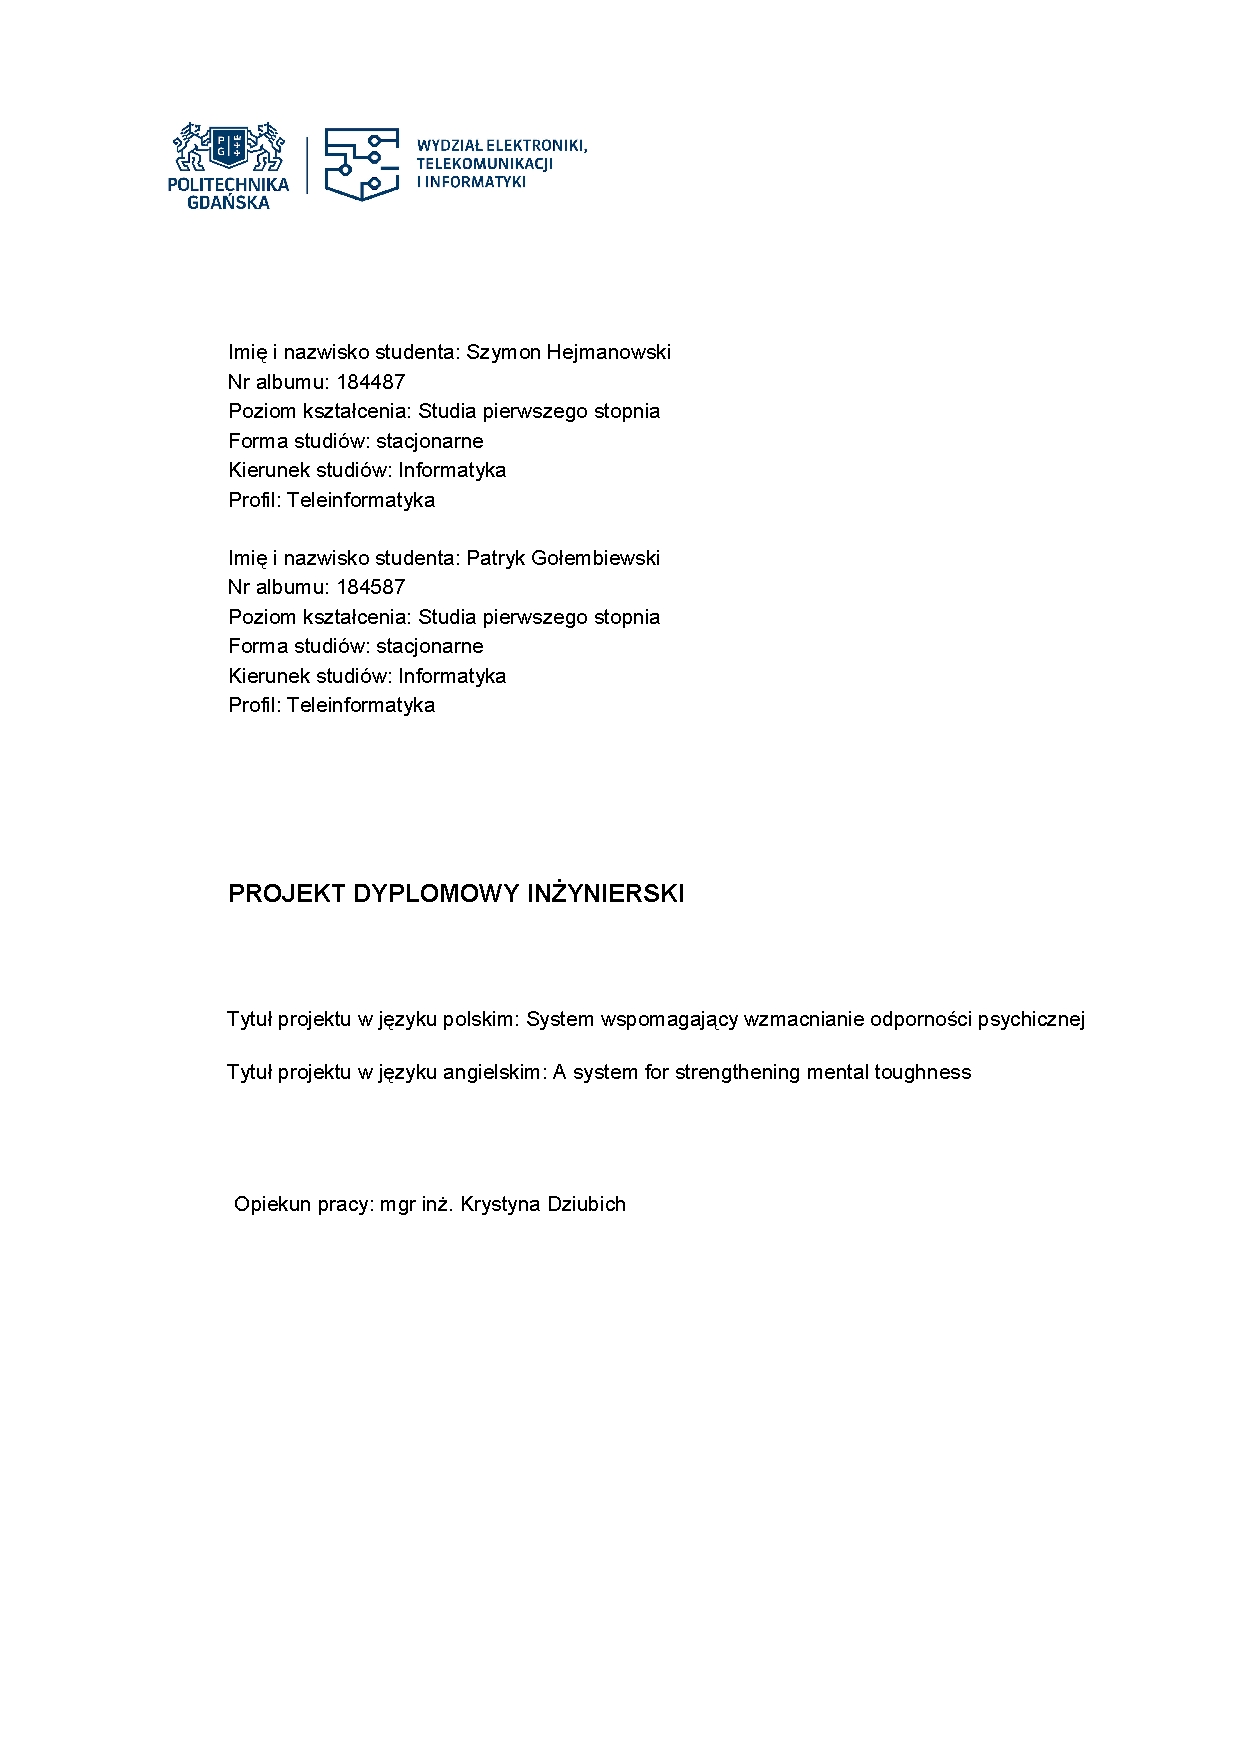
\includepdf{meta/strona_tytulowa.pdf}
%\includepdf{meta/oswiadczenie.pdf}

%------------------------------------------------------------
%  Dodanie streszczenia i abstract
%  						

\chapter*{Streszczenie}
\indent Lorem Lorem ipsum dolor sit amet, consectetur adipiscing elit. Vivamus elementum arcu nec blandit aliquam. Integer eros dolor, molestie eget dictum quis, luctus sit amet sapien. Proin dignissim felis in ornare volutpat. Morbi vulputate rutrum efficitur. Ut vehicula vehicula metus, et iaculis tortor mattis vel. Nam blandit, arcu quis ultricies blandit, libero ante commodo augue, in accumsan dui leo at orci. Phasellus in augue et velit pulvinar malesuada ut et sem. Nulla vehicula nibh eu odio sollicitudin sagittis. Praesent condimentum semper neque, tincidunt luctus nisl scelerisque sed. Orci varius natoque penatibus et magnis dis parturient montes, nascetur ridiculus mus. 
\vspace{0.5cm}\newline
\textbf{Słowa kluczowe:} lorem ipsum, dolor sit amet, consectetur adipiscing\vspace{0.5cm}

\noindent \textbf{Dziedzina nauki i techniki, zgodnie z wymogami OECD:} nauki inżynieryjne i techniczne, robotyka i automatyka

\chapter*{Abstract}
\indent This paper describe.... Lorem ipsum dolor sit amet, consectetur adipiscing elit. Vivamus elementum arcu nec blandit aliquam. Integer eros dolor, molestie eget dictum quis, luctus sit amet sapien. Proin dignissim felis in ornare volutpat. Morbi vulputate rutrum efficitur. Ut vehicula vehicula metus, et iaculis tortor mattis vel. Nam blandit, arcu quis ultricies blandit, libero ante commodo augue, in accumsan dui leo at orci. Phasellus in augue et velit pulvinar malesuada ut et sem. Nulla vehicula nibh eu odio sollicitudin sagittis. Praesent condimentum semper neque, tincidunt luctus nisl scelerisque sed. Orci varius natoque penatibus et magnis dis parturient montes, nascetur ridiculus mus. 
\vspace{0.5cm}\newline
\textbf{Keywords:} lorem ipsum, dolor sit amet, consectetur adipiscin \vspace{0.5cm}

%------------------------------------------------------------
%	Utworzenie spisu tre�ci pracy dyplomowej
\tableofcontents

%------------------------------------------------------------
%	Dodanie wykazu wazniejszych skr�t�w i oznacze� 
\chapter*{Wykaz ważniejszych oznaczeń i skrótów} % section* - ukrywa numerowanie oraz wyklucza ze spisu tresci
\addcontentsline{toc}{chapter}{Wykaz ważniejszych oznaczeń i skrótów}% % reczne dodanie do spisu tresci
\noindent PWM -- Pulse Width Modulation\newline
ADC -- Analog-to-Digital Converter \newline
SPI -- Serial Pheripheral Interface\newline
PCB -- Printed Circuit Board\newline


%------------------------------------------------------------
%	Dodanie rozdzia��w pracy dyplomowej - g��wne cia�o dokumentu 

\chapter{Wstęp i cel pracy}
ad
\chapter{Analiza merytoryczna}
W celu stworzenia optymalnego narzędzia pierwszym krokiem, przed zagłębieniem
się w aspekty techniczne, było przygotowanie się od strony merytorycznej. Aby
stworzyć aplikację, która będzie zgodna z naszymi założeniami, zgłębiliśmy
wiedzę w dziedzinie psychologi pod kątem odporności psychicznej oraz
prześledziliśmy podobne aplikacje dostępne na rynku. Uzbojeni w nową wiedzę
zastosowaliśmy wybrane metody kreatywności aby usprawnić proces tworzenia
pomysłów oraz wizji aplikacji. Przeprowadziliśmy dodatkowo badanie ankietowe
osób, które korzystały z podobnych narzędzi, co dało nam dodatkową perspektywę
oraz pomysły na naszą aplikację. Ostatecznie dzięki wszystkim wymienionym
procesom, stworzyliśmy wizję realizowanego systemu.
\section{Odporność psychiczna}
Odporność psychiczna, zwana również twardością, wytrzymałością lub rezyliencją
to cecha, która jest bardzo ceniona. Osoba, która posiada tę cechę, ma zdolność
wytrwania w trudnych sytuacjach i skupienia się na zadaniu. Wytrzymałość
psychiczna nie jest czymś, z czym się człowiek rodzi, raczej jest rozwijana i
doskonalona z biegiem czasu poprzez doświadczenia i wyzwania, które testują
granice naszej odporności. Utrzymanie pozytywnego nastawienia i umiejętność
dostosowania się do zmieniających się okoliczności to kluczowe czynniki w
budowaniu odporności psychicznej. Ostatecznie wytrzymałość psychiczna jest tym,
co odróżnia tych, którzy odnoszą sukcesy, od tych, którym się to nie udaje.

Stosowanie skutecznych strategii radzenia sobie w różnych sytuacjach może pomóc
nam wzmocnić naszą odporność psychiczną, która jest niezbędnym narzędziem w
pokonywaniu trudności i przeciwności losu. Nie wszyscy rodzimy się z takim samym
poziomem odporności psychicznej, ale ta cecha nie zależy wyłącznie od naszych
wrodzonych cech charakteru czy predyspozycji genetycznych. Poprzez praktykę i
naukę możemy rozwinąć naszą odporność psychiczną i stać się bardziej zdolni do
znoszenia życiowych trudności. Potwierdzają to swoimi słowami psycholog oraz
psychoterapeuta z wieloletnim doświadczeniem - Aleksandra Baca-Marzecka opisała
\textit{"Badacze uważają odporność psychiczną za cechę osobowości warunkowaną
genetycznie, którą jednak można modyfikować przez doświadczenie oraz
wykształcanie pewnych nawyków. Siła i odporność psychiczna nie są stałe, można
je rozwijać w zasadzie w każdym wieku"}\cite{Rymkiewicz}.

Dbanie o zdrowie psychiczne i budowanie odporności psychicznej stało się
najwyższym priorytetem w dzisiejszym zabieganym i stresującym świecie. Ponieważ
stres i napięcie są powszechnymi zjawiskami, skupienie się na zdrowiu
psychicznym stało się kluczowym tematem. Osoby o silnej odporności psychicznej
są lepiej przygotowane do radzenia sobie z problemami, są mniej podatne na
stres, lepiej radzą sobie z emocjami i relacjami z innymi oraz odnoszą większe
sukcesy w osiąganiu swoich celów. Mówiąc o odporności psychicznej, nie można nie
wspomnieć o \textbf{modelu 4C}, który definuje jej najważniejsze składniki.
Model 4C składa się z czterech filarów:

\begin{itemize}
    \item \textbf{Wyzwanie} (ang. challenge) - oznacza, że powinniśmy postrzegać
          trudności i wyzwania jako szanse do rozwoju i nauki, a nie jako
          problemy i przeszkody. Wyzwania stymulują rozwój i umożliwiają nam
          wzmocnienie swojej odporności psychicznej, dzięki czemu jesteśmy w
          stanie radzić sobie z przeciwnościami losu. Istotne jest, abyśmy
          traktowali problemy jako okazje do wzmocnienia swojej odporności
          psychicznej i szansę do rozwoju.
    \item  \textbf{Pewność siebie} (ang. confidence) - jest ona kluczowa dla
          budowania odporności psychicznej, ponieważ pomaga nam w radzeniu sobie
          z trudnymi sytuacjami i wyzwaniami. Posiadanie silnej pewności siebie
          oznacza, że jesteśmy przekonani o swoich umiejętnościach, zdolnościach
          i wartości, co pozwala nam na radzenie sobie z przeciwnościami losu
          bez utraty poczucia własnej wartości.
    \item \textbf{Zaangażowanie} (ang. commitment) - oznacza, że jesteśmy gotowi
          do poświęceń i pracy w celu osiągnięcia swoich celów. W kontekście
          budowania odporności psychicznej, oznacza to, że jesteśmy skłonni do
          regularnej pracy nad sobą, rozwoju i poszukiwania nowych umiejętności,
          co przekłada się na naszą zdolność do radzenia sobie z
          przeciwnościami.
    \item \textbf{Kontrola / poczucie wpływu} (ang. control) - oznacza, że mamy
          wpływ na swoje życie i decyzje. Poczucie kontroli nad własnym życiem
          wpływa na naszą zdolność do radzenia sobie z trudnościami i
          wyzwaniami, ponieważ daje nam poczucie pewności i siły. Istotne jest,
          abyśmy mieli poczucie kontroli nad swoim życiem, abyśmy czuli się w
          stanie wpływać na swoją sytuację życiową.
\end{itemize}

\begin{center}
    \textit{"To właśnie percypowanie nowych wyzwań jako potencjalnych szans na
        odniesienie sukcesu (wyzwanie), wiara we własne siły i możliwości
        (pewność siebie), wytrwałość w dążeniu do wyznaczonego celu
        (zaangażowanie) oraz poczucie realnego wpływu na swoje życie (kontrola)
        stanowią cztery filary (cztery razy C) ogólnej odporności psychicznej."}
        --- Małgorzata Ohme\cite{coaching}
\end{center}

\section{Podobne systemy}
Jednym ze sposobów wzmacniania odporności psychicznej jest korzystanie z
aplikacji dostępnych w Internecie. Szczególnie wygodne w użytkowaniu są systemy
dostępne na urządzeniach mobilnych. Dostepne są różne rozwiązania i
funkcjonalności, które pozytywnie oddziałują na samopoczucie człowieka i
radzenie sobie z trudnościami i wyzwaniami życiowymi, a także na rozwijanie
pewności siebie i umiejętności radzenia sobie ze stresem. W tym akapicie skupimy
się na omówieniu podobnych systemów i aplikacji, które zostały stworzone w celu
wzmacniania odporności psychicznej i pomagają w osiągnięciu lepszej jakości
życia. Przeanalizowane zostały aplikacje takie jak:

\begin{itemize}
    \item Personal Zen\footnote{https://personalzen.com/},
    \item
          Breath2Relax\footnote{https://apps.apple.com/us/app/breathe2relax/id425720246},
    \item Sanvello\footnote{https://www.sanvello.com/},
    \item
          Serenita\footnote{https://apps.apple.com/us/app/serenita-stress-anxiety/id954746715},
    \item Woebot\footnote{https://woebothealth.com/},
    \item
          Fitbit.\footnote{https://apps.apple.com/us/app/fitbit-health-fitness/id462638897}
\end{itemize}
Poniżej znajdują się opisy każdej z nich.


\textbf{Personal Zen} to aplikacja mobilna zaprojektowana specjalnie dla osób
doświadczających stresu i lęku. W ramach głównej praktyki użytkownicy codziennie
sprawdzają poziom stresu i nastroju. Na podstawie opinii aplikacja ustala
spersonalizowany cel, na przykład zalecaną liczbę minut grania dla danego
użytkownika, zazwyczaj od 5 do 10 minut dziennie. W grze pojawiają się dwa duchy
- przyjacielski i zły. Użytkownikom zaleca się podążanie ścieżką stworzoną przez
dobrego ducha. Użytkownicy powtarzają to ćwiczenie, aż osiągną swoje codzienne
cele. Inne funkcje aplikacji obejmują dziennik nastroju i treści
psychoedukacyjne.

\begin{figure}[h]
    \centering
    \subfloat[Główny ekran aplikacji]
    { \resizebox{0.4\textwidth}{!}{
            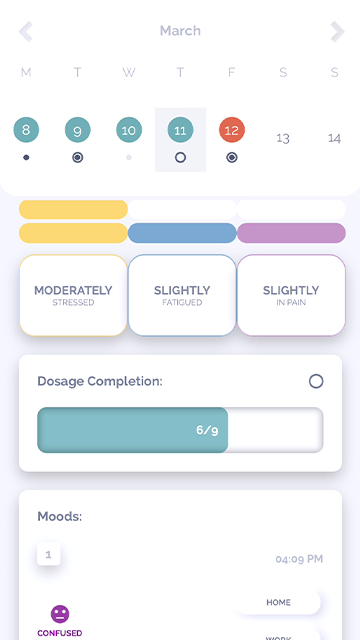
\includegraphics{img/zen.jpg}
        } } \subfloat[Moduł refleksji]{ \resizebox{0.4\textwidth}{!}{
            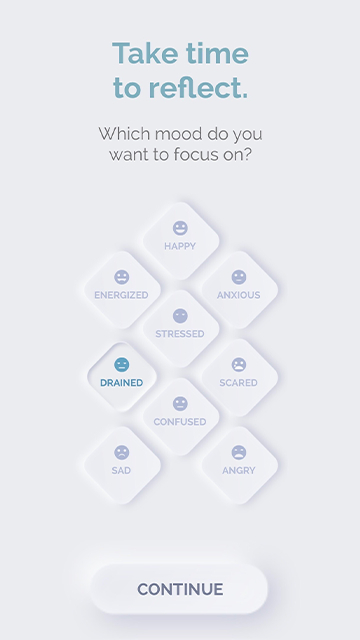
\includegraphics{img/zen2.jpg}
        } }
    \caption{Zrzuty ekranu z aplikacji Personal Zen}
\end{figure}

\textbf{Breathe2Relax} to darmowa mobilna aplikacja z dziedziny zdrowia i
fitnessu. Zawiera ona ćwiczenie prowadzonego oddechu przeponowego oraz przydatne
informacje na temat wpływu stresu.  Taka forma pracy z oddechem związana jest
często z praktyką mindfulness.

\textbf{Sanvello}, zarówno aplikacja internetowa, jak i mobilna, oferuje
użytkownikom ulgę od negatywnych emocji, takich jak niepokój, depresja i stres.
Wykorzystując strategie wywodzące się z terapii poznawczo-behawioralnej,
medytacji uważności, relaksacji i śledzenia nastroju/zdrowia, Sanvello oferuje
podejście oparte na dowodach. Ten program zaspokaja potrzeby użytkownika,
dostosowując swoje rekomendacje na podstawie generowanych raportów i
preferencji. Po zarejestrowaniu się Sanvello żąda aktualizacji aktualnego stanu
użytkownika, w tym nastroju, stanu zdrowia i celów, dostarczając precyzyjnych
zaleceń dotyczących określonych działań. Aplikacja oferuje różnorodne opcje, od
wielodniowych ścieżek samopomocy z przewodnikiem, po techniki relaksacyjne, a
nawet czaty grupowe.

\begin{figure}[h]
    \centering
    \subfloat[Ekran wyboru modułu]
    { \resizebox{0.4\textwidth}{!}{
            
\includegraphics{img/senvello.jpg}
        } } \subfloat[Ekran z poradnikami]{ \resizebox{0.4\textwidth}{!}{
            
\includegraphics[]{img/senvello2.jpg}
        } }
    \caption{Zrzuty ekranu z aplikacji Senvello}
\end{figure}
Dzięki \textbf{Serenicie} użytkownicy mogą bez wysiłku zarządzać i śledzić
poziom stresu. Aby ocenić poziom stresu, aplikacja wykorzystuje aparat telefonu
w funkcji „Stress Check”. Aby zredukować stres lub zwiększyć koncentrację,
Serenita zapewnia różnorodne ćwiczenia. Aktywność Interaktywna Relaksacja
rozpoczyna się od pomiaru poziomu stresu i wzorców oddychania za pomocą
50-sekundowego testu stresu. Podczas ćwiczenia oddechowego obecny jest wizualny
przewodnik, który instruuje użytkownika, kiedy należy wdychać, wstrzymywać i
wydychać powietrze. Po pomyślnym ukończeniu ćwiczenia oddechowego użytkownik
otrzymuje punkty. Korzystając z innego wzorca oddychania, ćwiczenie Interaktywne
Skupienie zostało zaprojektowane w celu zwiększenia skupienia. Długość ćwiczeń
można dostosować do własnych potrzeb, do 5 minut. Po wykonaniu ćwiczenia
aplikacja dostarcza informacji o wzroście lub spadku poziomu stresu w całym
ćwiczeniu. Funkcja "trend" dostarcza wykres postępu użytkownika na każdym
ćwiczeniu w czasie. Dostępnych jest pięć sesji każdego ćwiczenia, które zawarte
zostały w bezpłatnej wersji aplikacji.

\textbf{Woebot} jest w pełni zautomatyzowanym agentem konwersacyjnym. Woebot
jest dostępny za pośrednictwem urządzeń mobilnych poprzez aplikację
komunikatora. Aplikacja zawiera lekcje, interaktywne ćwiczenia i filmy wideo
oparte na terapii poznawczo-behawioralnej. Interakcje z Woebotem są dosyć
krótkie (1-2 minuty). Istnieje jednak możliwość wydłużenia sesji.

Poniższy fragment przedstawia zestawienie aplikacji oraz funkcjonalności, które
najczęściej w nich występowały. Opis funkcjonalności przytaczanych w tabeli:
\begin{itemize}
    \item Dziennik - zapisuje się w nim codzienny nastrój i poziom stresu.
    \item Gra - prosta w założeniu, pomaga uspokoić myśli i na chwilę się na
          czymś skupić.
    \item Oddech - instruktor oddechu, ułatwia uspokojenie się i wejście w stan
          medytacji
    \item Ćwiczenia - lista ćwiczeń dobranych tak, aby pomagały w relaksacji.
    \item Chatbot - czat AI z którym możemy pogadać.
    \item Sen - pomaga wyregulować godziny snu i poprawić jego jakość.
\end{itemize}

\begin{table}[h]
    \small
    \centering
    \begin{tabular}{ | c | c | c | c | c | c | c | }
        \hline
                     & Dziennik & Gra & Oddech & Ćwiczenia & Chatbot & Sen \\
        \hline
        Personal Zen & +        & +   &        &           &         &     \\
        \hline
        Breath2Relax &          &     & +      &           &         &     \\
        \hline
        Sanvello     & +        &     & +      & +         &         &     \\
        \hline
        Serenita     & +        & +   & +      &           &         &     \\
        \hline
        Woebot       & +        &     &        &           & +       &     \\
        \hline
        Fitbit       & +        & +   &        &           &         & +   \\
        \hline
    \end{tabular}
    \caption{Porównanie funkcji podobnych systemów}
\end{table}

\pagebreak

Po przeanalizowaniu powyższych oraz innych aplikacji, autorom nastunęły się
następujące refleksje. Użytkownik ma dostęp do wielu różnych rozwiązań, jednak
wiele z nich posiada funkcjonalności nie wpływające bezpośrednio na zwiększenie
odporności psychicznej. Przykładem są gry, które odciągają uwagę odbiorcy od
złych myśli. Pozwalają one jedynie na chwile zapomnieć o problemach, jednak gdy
użytkownik przestanie używać tego modułu, problemy wracają. Ponownie musi wrócić
do świata rzeczywistego i zderzyć się ze swoimi problemami. Kolejnym
spostrzeżeniem jest możliwa wadliwość sztucznej inteligencji w sprawach
emocjonalnych i szeroko rozumianej psychiki człowieka. Czatbot może mieć
trudności w zrozumieniu kontekstu rozmowy, co może prowadzić do błędów
interpretacyjnych i nieodpowiednich odpowiedzi, a w skutku, negatywnie odbić się
na użytkowniku. Inna wadą jest brak różnorodności w ćwiczeniach. Choć aplikacja
oferuje interesujące i skuteczne ćwiczenia, to po pewnym czasie użytkownicy mogą
się nudzić i potrzebować czegoś nowego, aby utrzymać swoją motywację do
korzystania z aplikacji. Przykładowo Personal Zen oferuje tylko jedno główne
ćwiczenie, co może być niewystarczające dla niektórych użytkowników. Brak nowych
treści lub różnorodnych ćwiczeń może skutkować tym, że użytkownicy przestaną
korzystać z aplikacji lub szukają innych aplikacji, które oferują więcej
różnorodności.

\section{Zastosowane metody kreatywności}

Tworzenie aplikacji mającej na celu poprawę odporności psychicznej to proces
wymagający wykorzystania różnych narzędzi i technik. Jednym z kluczowych
aspektów jest kreatywność, która pozwala na generowanie nowych pomysłów i
podejście do projektu z różnych perspektyw. W celu zwiększenia kreatywności, w
ramach pracy inżynierskiej zastosowaliśmy trzy różne metody, a mianowicie:
scenariusze użycia, mapę empatii oraz negatywnej burzy mózgów. Ich wykorzystanie
miało na celu uzyskanie bardziej wartościowych i innowacyjnych rozwiązań, które
są dostosowane do potrzeb i oczekiwań użytkowników. W dalszej części rozdziału
przedstawione zostaną szczegółowe informacje na temat każdej z tych metod, wraz
z opisem ich zastosowania w projektowaniu aplikacji.

\subsection{Scenariusze użycia}
Metoda scenariuszy użycia to podejście projektowe polegające na stworzeniu
szczegółowych opisów procesów, jakie użytkownicy będą wykonywać przy korzystaniu
z danego produktu lub usługi. Polega ona na identyfikacji problemów, jakie mogą
napotkać użytkownicy w trakcie interakcji z systemem, a następnie na opracowaniu
sposobów, w jaki te problemy mogą zostać rozwiązane. Scenariusze użycia mogą być
tworzone na różnych etapach projektowania, a ich celem jest poprawa użyteczności
i łatwości korzystania z danego systemu.

W przypadku naszego projektu scenariusze użycia były stworzone w formie tabeli z
kolumnami \textbf{AS IS} oraz \textbf{TO BE}. Do jednej kolumny, oznaczonej jako
AS IS, wpisane zostały opisy sytuacji w jakich może znajdować się osoba z
problemami na podłożu odporności psychicznej. Kolumna TO BE, zawiera z kolei
scenariusz, w którym z wykorzystaniem naszej aplikacji osoba radzi sobie z danym
problemem. Za pomocą tej metody stworzyliśmy opisy sytuacji, zawierające zbiór
pomysłów na funkcjonalności jakie moglibyśmy zaimplementować w naszej aplikacji.
Pomogło to nam w procesie generowania funkcji systemu oraz zobrazowało które z
pomysłów mają praktyczne zastosowanie. Poniżej znajduje się zbiór zestawień AS
IS oraz TO BE scenariuszy użycia:
\begin{itemize}
    \item \textbf{AS IS I} Osoba szybko zniechęca się do wykonywanych zadań,
          ponieważ nie czuje namacalnego progresu. Przez to, że myśli jedynie o
          tym co ma jeszcze do wykonania (a nie odnotowuje ile już zrobiła) ma
          ciągłe wrażenie braku postępu, co ją wysoce demotywuje. Brak kontroli
          oraz zaangażowania.
    \item \textbf{TO BE I} Osoba dzięki aplikacji i zapisywaniu każdego zadania
          może w każdej chwili sprawdzić ile już zrobiła, dzięki temu czuje
          progres co motywuje ją do dalszego działania. „Odhaczanie” kolejnego
          zadania z listy, powoduje malutki zastrzyk dopaminy, co w długim
          terminie tworzy w mózgu połączenia łączące wykonywanie kolejnych zadań
          z przyjemnością.
    \item \textbf{AS IS II} Osoba nie ma jasno wyznaczonych i skonkretyzowanych
          celów do jakich dąży. Chce schudnąć jednak nigdzie nie odnotowała ile
          i w jakim czasie. Przez to, że cel jest bardzo ogólny i bez
          wyznaczonego terminu, jest on tak naprawdę jedynie marzeniem. Osobie
          tej, wydaje się, że od czasu do czasu zje mniej lub pójdzie pobiegać,
          więc dąży do realizacji celu, jednak nie zdaje sobie sprawy, że
          wykonywana praca jest wyraźnie zbyt mała aby odnieść rezultat. Tkwi w
          przekonaniu, że dąży do celu, jednak w rzeczywistości jedynie stoi w
          miejscu. Taki status quo w dziedzinie jej celów obniża jej pewność
          siebie, ma wrażenie, że jest gorsza od innych bo też pracuje, jednak
          bez rezultatu. Dodatkowo traci poczucie kontroli, ma wrażenie, że nie
          ma wpływu na to co się dzieje w jej życiu. Nie jest w stanie realnie
          się zaangażować. Również taki stan ne- gatywnie wpływa na obszar
          wyzwań z modelu 4C – nigdy nie ponosi jednoznacznej porażki (ponieważ
          jej cel nie ma terminu ani konkretnych założeń), z której mogłaby
          wyciągnąć lekcje, a jednocześnie nigdy nie osiąga celu.
    \item \textbf{TO BE II} Osoba dodaje nowy cel w aplikacji zgodnie z
          formularzem. Podaje tam obiektywne i mierzalne wartości, które chce
          osiągnąć (konkretna waga, ilość pieniędzy jakie chce zarobić, ilość
          materiału do nauczenia) oraz termin realizacji tych zadań. W obszarze
          celu może również ustawić tak zwane milestones, czyli cele pośrednie,
          które są kluczowe do osiągnięcia ostatecznego celu. Widok bliższego
          celu pośredniego na horyzoncie daje jej dużą motywacje na początku i
          podtrzymuje ją w momentach zwątpienia. Osoba ta ma realne cele i w
          pełni świadomie dąży do nich każdego dnia. Osoba widząc postęp w
          kolejnych celach zyskuje poczucie kontroli nad sobą oraz własnym
          życiem. Pozwala jej się to również zaangażować i trwać w swoich
          postanowieniach. Jeśli któregoś z celów nie wypełni, zdaje sobie
          sprawę ze swojej porażki co pozwala jej wyciągnąć lekcje, wpływa to
          dobrze na obszar Wyzwania. Większa kontrola oraz widoczny rozwój
          zwiększa jej pewność siebie i przekłada się pozytywnie na inne ob-
          szary.
    \item \textbf{AS IS III} Osoba ma skłonności do pesymizmu, lubi się
          zamartwiać i znajdować we wszystkim jedynie negatywy. Jest to dla niej
          demotywujące i zabija w niej chęć rozwoju. Osoba twierdzi, że rozwój i
          tak nic nie zmieni i że w ogóle jest bezsensu.
    \item \textbf{TO BE III} Aplikacja zapewnia osobie codzienne cytaty
          motywujące oraz inspirujące myśli tych, którzy wiele osiągnęli. O ile
          nie wpływa to z dnia na dzień na osobę, to jednak w dłuższym okresie
          czasu pozwala jej unikać pułapki ciągłego pesymizmu i odżywia jej mózg
          pozytywnymi myślami.
    \item \textbf{AS IS IV} Osoba przez lata złych nawyków kształtowanych przez
          system szkolny oraz własne zaniedbania ma duże problemy ze snem. Nie
          zdaje sobie sprawy z tego, na jak wiele obszarów zdrowia oraz pracy
          mózgu on wpływa. Zaniedbuje sen sypiając w różnych godzinach oraz
          często niewystarczająco długo. Ma problemy z przyswajaniem i
          zapamiętywaniem, również pamięć mięśniowa na tym traci, przez co np.
          nauka gry na fortepianie staje się dla niej dużo trudniejsza. Odczuwa
          również negatywne skutki słabej higieny snu poprzez częste
          przeziębienia. Nierzadko musi odpuszczać przez to treningi lub wyjścia
          ze znajomymi. Ma poczucie braku kontroli nad własnym zdrowiem.
          Dodatkowo trudności w przyswajaniu informacji oraz w nauce nowych
          czynności fizycznych zmniejszają jej pewność siebie.
    \item \textbf{TO BE IV} Dzięki modułowi poprawy snu osoba może dowiedzieć
          się o tym jak ogromne skutki ma jego zaniedbywanie. Dzięki przejrzeniu
          panelu poświęconemu krótkim informacją z badań o negatywnych skutkach
          niepoprawnego snu znajduje potencjalne rozwiązanie swoich wielu
          problemów. Motywuje ją to do działania w tym obszarze życia. Ustala w
          aplikacji harmonogram snu, co skutkuje codziennymi przypomnieniami
          i/lub blokowaniem innych aplikacji w odpowiednich godzinach. Sprawdza
          również panel zapewniający krótkie porady o tym jak zadbać o dobrą
          jakość snu (zmniejszenie temperatury pokoju, przygotowanie do snu
          poprzez zmniejszenie tętna). Poprawa ilość oraz jakości snu wpływa
          pozytywnie na każdy aspekt życia osoby. Lepiej działający układ
          immunologiczny redukuje czę- sto liczbę przeziębień, dzięki czemu
          osoba nie musi opuszczać treningów i innych aktywności. Osoba
          przyswaja więcej materiału i pamięta go lepiej, co również redukuje
          czas jaki musi poświęcać na naukę. Dodatkowo nauka gry na fortepianie
          idzie nagle zauważalnie lepiej. Osoba zyskuje pewność siebie oraz
          poczucie kontroli nad własnym życiem i zdrowiem. 10
    \item \textbf{AS IS V} Osoba ma problemy ze skupieniem. W każdej wolnej
          chwili przegląda social media lub ogląda seriale. Nie pozostawia jej
          to praktycznie żadnego czasu na uspokojenie myśli. Jedyny czas kiedy
          jest sama ze swoimi myślami to moment kiedy kładzie się spać. Nie
          pozwala jej to wyłączyć się i spokojnie zasnąć. Skupienie się przez
          dłuższy moment na pracy głębokiej lub na czynności nie dostarczającej
          do mózgu dużych ilości bodźców jest dla niej praktycznie nie- realne.
          Przy nudnych aktywnościach odruchowo co chwilę sięga po telefon.
          Podczas czytania książki, osoba się irytuje, musi wielokrotnie czytać
          każde zdanie ponieważ co chwilę jej myśli pędzą w inną stronę. Ciągła
          praca mózgu na wysokich obrotach powoduje u osoby niepokój. Nie jest
          nawet do końca świadoma z czego on wynika, jednak wyraźnie go odczuwa
          z różną intensywnością na przestrzeni dnia. Osoba taka nie ma poczucia
          kontroli nawet nad własnymi myślami. Nie jest w stanie zaangażować się
          w pracę którą wykonuje.
    \item \textbf{TO BE V} Dzięki użytkowaniu aplikacji z wyszczególnieniem
          modułu medytacji / pracy nad oddechem, osoba zaznaje każdego dnia
          parunastu minut uspokojenia myśli. Jest w stanie codziennie pracować
          nad swoją uważnością. W jej głowię zaczynają pojawiać się nowe myśli.
          Po pewnym okresie codziennej medytacji niepokój osoby stopniowo
          zanika, jest ona w stanie o wiele łatwiej i lepiej skupić się na
          wykonywanych czynnościach. Często zdarza jej się wchodzić w tryb
          „flow”. Czynności której wcześniej wydawały się nudne (np. czytanie
          książki), teraz sprawiają jej przyjemność. Na co dzień nie ma wrażenie
          ciągłej gonitwy myśli, jest w stanie być bardziej obecna w danej
          chwili. Spokojny i uważny umysł pozytywnie przekłada się również na
          zasypianie. Przed snem osoba korzystając z aplikacji uspokaja myśli i
          kładzie się do snu w idealnym stanie. Osoba zyskuje dużo lepsze
          poczucie kontroli oraz jest w stanie angażować się w codzienne
          wyzywania.
    \item \textbf{AS IS VI} Osoba przechodzi przez każdy kolejny dzień bez
          refleksji, nie zwraca uwagi na to jakie wydarzenia z dnia wpływają na
          jej samopoczucie. Często popełnia te same błędy ponieważ nie poświęca
          czasu na przemyślenie ich i znalezienie rozwiązania. Nie jest do końca
          świadoma swoich własnych emocji. Wraca w głowie do przeszłości jednak
          nie w celu jej analizy i wyciągnięcia wniosków, lecz w celu rozmyślań
          nad tym co by było gdyby postąpiła inaczej. Tworzy w ten sposób
          negatywne nastawienie do swojej własnej osoby jednocześnie nic nie
          zyskując. Traci pewność siebie.
    \item \textbf{TO BE VI} Osoba z użyciem aplikacji poświęca codziennie chwilę
          by przeanalizować miniony dzień. Zapisuje problemy jakie wystąpiły
          danego dnia oraz znajduje ich rozwiązania / sposoby na uniknięcie w
          przyszłości. Jeśli dany problem pojawiał się kolejny raz, myśli nad
          tym dlaczego poprzednie rozwiązanie było nieskuteczne i jak je
          poprawić / zmienić. Ocenia również swoje samopoczucie na koniec dnia,
          dzięki czemu zyskuje świadomość co tak naprawdę wpływa na jej
          odczucia. Dzięki widocznej eliminacji błędów oraz świadomości emocji
          czuje, że zyskuje pewność siebie oraz kontrole.
    \item \textbf{AS IS VII} Osoba każdego dnia budzi się bez konkretnych
          założeń co do tego co chciałaby zrobić. Ma w głowie zarys planów na
          dzień, jednak są one nieskonkretyzowane. W dni w które ma wiele zadań
          nie czuje potrzebnej presji, przez co dzień nie jest optymalny i nie
          wyrabia się ze zrobieniem wszystkiego co powoduje stres i
          niezadowolenie. W dni, kiedy ma mało zadań i dużo czasu, zamiast
          skorzystać z możliwości i zaplanować ciekawą aktywność na ten dzień
          lub wykonać jakąś pracę na zapas, traci pół dnia na bezproduktywne
          czynności. Nie ma poczucia kontroli nad własnym dniem, nie jest w
          stanie optymalnie wykonywać swoich wyzwań oraz nie jest tak
          zaangażowana jakby mogła być.
    \item \textbf{TO BE VII} Osoba codziennie wieczorem po wypełnieniu dziennika
          samopoczucia przechodzi do sekcji planowania następnego dnia. Na
          spokojnie zbiera wszystkie rzeczy, które powinna jutro zrobić i tworzy
          z nich listę. Nadaje im priorytety, szacunkowy czas wykonania oraz
          godziny. Widzi czy jest na nie- doczasie i musi jutro wyjątkowo się
          wysilić czy może ma trochę wolnego czasu aby wyjść na kawę ze
          znajomymi. Następnego dnia od rana skoncentrowana jest na wypełnianiu
          zadań. Daje jej to duże poczucie satysfakcji co ułatwia przystępowanie
          do kolejnych zadań. Dzięki przydziałowi na każde zadanie swojego czasu
          jest w stanie skupić się na obecnie wykonywanej czynności. Dodatkowo
          świadomość na jakim etapie pracy jest w ciągu dnia redukuje w dużym
          stopniu jej stres i niepokój. Odhaczenie ostatniego zadania w trakcie
          danego dnia powoduje wyrzut dopaminy i zachęca do powtórzenia cyklu
          dnia kolejnego.
\end{itemize}


\subsection{Mapa empatii}
Drugą metodą kreatywności, którą zastosowaliśmy, jest mapa empatii. Jest to
narzędzie, które pozwala na lepsze zrozumienie potrzeb i oczekiwań użytkowników.
Polega ona na stworzeniu mapy, na której umieszczamy informacje na temat
użytkowników, ich myśli, emocji, działań oraz otoczenia. Dzięki temu, możemy
uzyskać bardziej szczegółowe informacje na temat użytkowników i ich potrzeb, a
także wykorzystać te informacje do tworzenia bardziej wartościowych rozwiązań.
Użyty przez nasz szablon mapy empatii został przedstawiony na Rysunku
\ref{mapa_empatii}.
\begin{figure}[h]
    \centering
    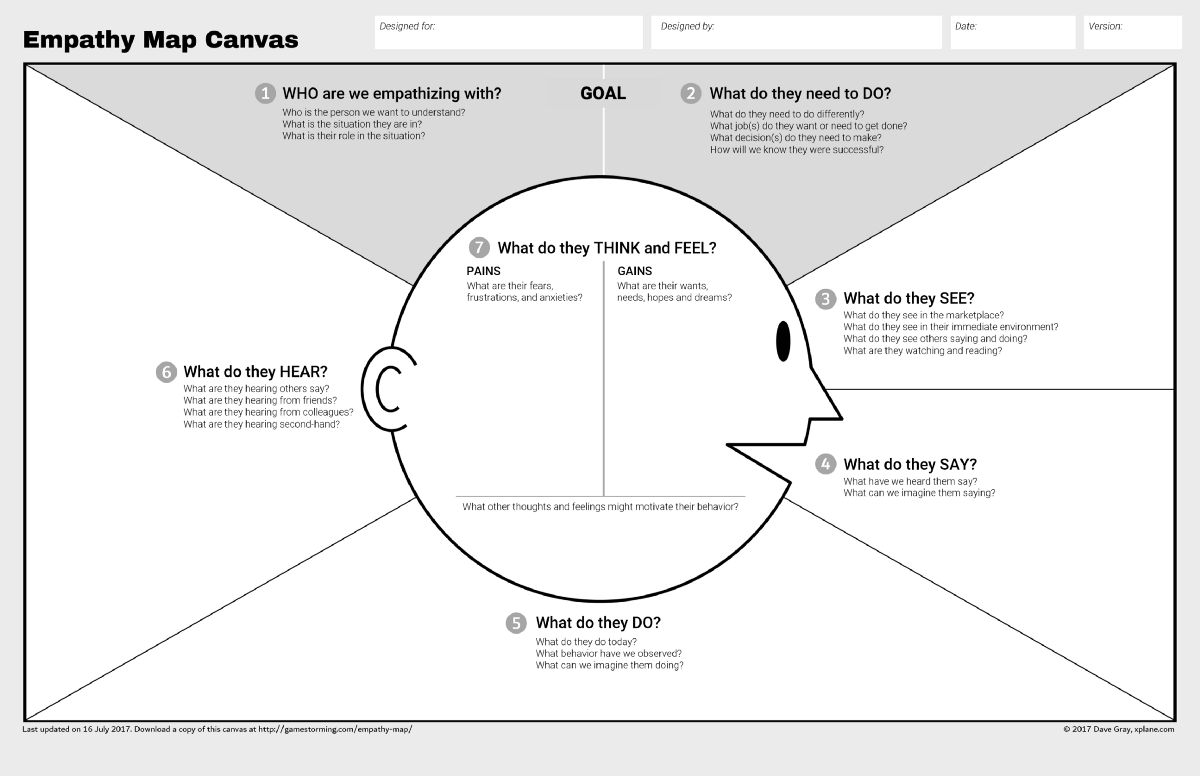
\includegraphics[width=\textwidth]{img/empathymap.png}
    \caption{Wykorzystany schemat mapy empatii}
    \label{mapa_empatii}
\end{figure}

\begin{itemize}
    \item \textbf{Kogo chcemy zrozumieć?} Osoba, która chce poprawić swoją
          odporność psychiczną. Osoba taka mierzy się na co dzień z wieloma
          wyzwaniami i problemami chce być w stanie zwalczać je z większą
          łatwością oraz mieć większy komfort psychiczny.
    \item \textbf{Co ta osoba musi zrobić?} Zapoznać się z aplikacją. Nauczyć
          się jej obsługi. Uzupełnić cele długoterminowe. Codziennie zaglądać do
          aplikacji, aby uzupełnić dziennik oraz wyznaczyć cele na kolejny
          dzień.
    \item \textbf{Co osoba widzi?} Na co dzień widzi świat pełen trudności i
          problemów. Niezliczoną ilość przytłaczających wyzwań. W Internecie
          widzi innych, którzy cieszą się życiem i wydają się nie posiadać
          żadnej troski. Widzi ciągłe zmiany do których nie jest w stanie
          przywyknąć oraz ludzi, z których każdy wydaje się obcy.
    \item \textbf{Co to osoba mówi?} Mówi, że nie jest w stanie sobie poradzić z
          codziennością. Narzeka na nieustające trudności. Mówi, że nie czuje
          kontroli nad własnym życiem.
    \item \textbf{Co ta osoba robi?} Stoi w miejscu, pragnąc zmiany. Nie jest w
          stanie jednak niczego wskórać. Codziennie obiecuje sobie, że
          zrealizuje postawione cele, jednak jest to tylko złudne poczucie.
          Każdego dnia idzie spać o innej porze, przez co nie jest w stanie się
          wyspać. Nie pielęgnuje relacji z bliskimi. Jest reaktywna, zarówno w
          życiu zawodowym jak i osobistym. Nie pomaga innym.
    \item \textbf{Co ta osoba słyszy?} Od innych słyszy, że musi wziąć się w
          garść i zrobić coś ze swoim życiem. Docierają do niej stale słowa
          krytyki od innych. Koledzy namawiają ją na wyjścia jednak ona nie ma
          siły ani ochoty wychodzić z domu.

    \item \textbf{Co ta osoba myśli i czuje?}
          \begin{itemize}
              \item \textbf{Bóle:} Ma lęk przed tym, że nie będzie w stanie
                    zrealizować wszystkich zadań oraz, że nie radzi sobie z
                    codziennymi problemami. Jest sfrustrowana swoją postawą i
                    ciągłym brakiem poprawy. Boi się, że przez swoje
                    zaniedbywanie kontaktów oraz złe nastawienie odwrócą się od
                    niej znajomi. Obawia się o swoje zdrowie fizyczne z powodu
                    zaniedbywania sfery somatycznej egzystencji.
              \item \textbf{Nadzieje:}  Ma nadzieję, że walka z codziennymi
                    trudnościami będzie dla niej łatwiejsza. Chciałaby z
                    uśmiechem stawiać czoła kolejnemu dniu. Zależy jej również
                    na poprawie relacji z ludźmi. Liczy, że jej zdrowie fizyczne
                    również się poprawi. Chciałaby mieć pełną kontrolę nad swoim
                    życiem oraz większą pewność siebie. Obecnie czuje złość, że
                    nie jest w stanie realizować swoich postanowień.
          \end{itemize}
\end{itemize}

\subsection{Negatywana burza mózgów}

Trzecią metodą kreatywności, którą wykorzystaliśmy, jest negatywna burza mózgów.
Jest to technika generowania pomysłów, która polega na znajdywaniu problemów,
aby móc im potem przeciwdziałać. Metoda ta pozwala na stworzenie listy
potencjalnych złych doświadczeń podczas korzystania z aplikacji. Dzięki temu,
pobudzamy wyobraźnię i wyzwalamy myślenie o niestandardowych rozwiązaniach. Była
to ostatnia z metod kreatywności jaką zastosowaliśmy, więc w tym przypadku
poprzednie metody kreatywności w dużym stopniu wypełniły analizowany obszar
systemu, jednak metoda negatywnej buzy mózgów miała na celu pomóc nam spostrzec
niektóre przeoczone aspekty tworzenia systemu. Celem było zwrócenie uwagi między
innymi na to, że aplikacja powinna być stworzona w taki sposób, aby korzystanie
z niej nie stawało się kolejnym czasochłonnym obowiązkiem w życiu danej osoby
oraz że, aby dana osoba korzystała z pełnym zaufaniem z metod zawartych w
aplikacji powinniśmy przedstawiać dowody naukowe popierające słuszność danej
funkcjonalności. Rezultaty zostały przedstawione w tabeli \ref{burza}.

\begin{table}[h]
    \centering
    \begin{tabular}{ | m{0.47\textwidth} | m{0.47\textwidth} | }
        \hline
        POTENCJALNE PROBLEMY                                      & ROZWIĄZANIE
        \\
        \hline
        Korzystanie z aplikacji zajmuje zbyt dużo czasu w ciągu dnia. Staje się
        to dodatkowym obowiązkiem.                                &
        Optymalizacja czasu który potrzebny jest na korzystanie z aplikacji.
        Stworzenie intuicyjnego UI.
        \\
        \hline
        Osoba przestaje używać aplikacji po krótkim czasie, ponieważ mija jej
        chwilowa motywacja.                                       &
        Powiadomienia przypominające o postępie w celach oraz hasła motywujące.
        \\
        \hline
        Bariera językowa. Osoba nie ma dostępnego swojego języka. & Aplikacja
        dostępna w języku Polskim oraz Angielskim. \\
        \hline
        Osoba nie jest przekonana co do metod wykorzystywanych w aplikacji, nie
        chce z nich korzystać ponieważ nie wie czy działają.      & W każdym
        module zawiera się panel z krótkim opisem na jakiej zasadzie działa dana
        funkcjonalność. Dodatkowo poparte są badaniami. \\
        \hline
        Osoba nie widzi postępu w swoich działaniach.             & Każdy panel
        ma swój pasek postępu i cele do wypełnienia. Np. medytuj 1000 razy \\
        \hline
    \end{tabular}
    \caption{Wnioski płynące z negatywnej burzy mózgów}
    \label{burza}
\end{table}

\section{Badania ankietowe}
Ankiety mają coraz większe znaczenie w dzisiejszych badaniach nad zdrowiem
psychicznym i zachowaniem. W kontekście aplikacji mobilnych, ankiety dotyczące
potrzeb użytkowników mogą dostarczyć cennych informacji na temat oczekiwań i
preferencji dotyczących narzędzi wspierających zdrowie psychiczne. Wyniki takich
badań mogą pomóc w projektowaniu i udoskonalaniu aplikacji, tak aby lepiej
odpowiadały na potrzeby użytkowników. Istnieje wiele różnych aplikacji
mobilnych, które mają na celu wspieranie zdrowia psychicznego, dlatego ankiety
mogą pomóc w unikaniu błędów oraz mankamentów występujących w istniejących
rozwiązaniach.

W początkowej fazie kwestionariusza zaczęliśmy od pytań odnośnie wzmacniania
odporności psychicznej. Większość ankietowanych jest zainteresowana wzmacnianiem
odporności oraz stara się aktywnie nad nią pracować. Jest to dobry znak, gdyż
nasza aplikacja mogłaby zostać jedną z możliwości dalszej pracy nad sobą dla
takich osób. Istnieje zatem potrzeba utworzenia takiego systemu. Następnie
ankietowani zostali zapytani o znajomość modelu 4c. Niestety okazuje się, że nie
do końca wiedzą czym on jest. Po zapoznaniu się z filarami tego modelu, mieli
oni wybrać najważniejszy z nich według ich uznania. Faworytami okazały się
pewność siebie oraz zaangażowanie. W kolejnym pytaniu odpowiedzi użytkowników
nawiązały do drugiego z wymienionych filarów. Uznali oni brak zaangażowania oraz
trzymanie się wyznaczonych celów za najtrudniejsze elementy życia codziennego -
\textit{"trzymanie się wyznaczonych przez siebie celów i kultywowanie zdrowych
nawyków […] systematyczność."}.

Następnym zagadnieniem poruszanym w ankiecie był pozytywny wpływ różnych rzeczy
na stan psychiczny. Analizując odpowiedzi doszliśmy do wniosku, że różne metody
poprawy odporności psychicznej działają na różne osoby w różny sposób. Wśród
najczęściej wymienianych sposobów na poprawę odporności psychicznej są poprawa
snu i diety, regularne ćwiczenia fizyczne, medytacja w celu wyciszenia i
zrozumienia własnych emocji oraz śledzenie postępu, aby widzieć progres i nie
tracić zaangażowania.

Ostatnia część dotyczyła aplikacji, które wzmacniają odporność psychiczną.
Ankietowani jednogłośnie uznali, że aplikacje mogą mieć duży wpływ na
zwiększanie odporności. W kolejnym pytaniu wymienili sposoby wpływania systemów
wspierających odporność psychiczną:
\begin{itemize}
    \item \textit{"Motywowanie do realizacji celów, uspokajanie."}
    \item \textit{"Poprzez dawanie porad jak i pomocnych zadań."}
    \item \textit{"Mogą pokazać, że jesteś w czymś stabilny lub zrobiłeś jakiś
              postęp względem przeszłości."}
    \item \textit{"[...] aplikacja, która pozwoli się na chwilę zatrzymać,
          przypomnieć o postawionych sobie celach i wyzwaniach, sprawdzić jakie
          robimy postępy."}
\end{itemize}
Użytkownicy napisali również powody, dla których wcześniej rezygnowali z
korzystania z podobnych aplikacji. Pojawiającą się odpowiedzią było rozbicie
funkcjonalności po różnych aplikacjach, a co za tym idzie szybkie zniechęcanie
się do nich. Pytaniem zwieńczającym ankietę była prośba o wypisanie
funkcjonalności, które wg ankietowanych będą użyteczne w aplikacji. Oto
przykładowe, najczęstsze odpowiedzi:
\begin{itemize}
    \item \textit{"Możliwość monitorowania progresu, system nagród"}
    \item \textit{"Dziennik codziennego stanu emocjonalnego, możliwość
              połączenia smartwatch z funkcją monitorowania stresu i
              monitorowanie wyników, motywowanie w osiąganiu celów - system
              nagród"}
    \item \textit{"Śledzenie postępu w postanowionych celach, instrukcje,
              poradniki mające na celu poprawić jakość snu, diety, zarządzanie
              czasem."}
\end{itemize}

\section{Wizja aplikacji}
Głównym założeniem naszej aplikacji jest poprawa odporności psychinczej jej
użytkowników. Poprzez działanie oparte na \textbf{modelu 4C} ma ona ułatwiać
wprowadzanie metod, pozytywnie wpływających na rezyliencje w codziennym życiu.
Chcemy aby aplikacja była bodźcem pozwalającym na systematyczny oraz przemyślany
rozwój psychiczny użytkownika. Dzięki dobraniu odpowiednich funkcjonalności oraz
ich przemyślanej implementacji, otrzymujemy produkt, który pozwala na optymalne
wprowadzenie nowych nowyków w życie każdego z nas.

Celem systemu jest pozytywna zmiana w życiu użytkownika. Aplikacja ma uczyć
nowych nawyków oraz pomagać wprowadzić je w życie. Dodatkowo jej celem jest
zmiana myślenia użytkownika oraz zwiększenie jego świadomości na tematy związane
z odpornością psychiczną.

Nasz system będzie przeznaczony dla szerokiego spektrum użytkowników, w tym dla
studentów, pracowników biurowych oraz rodziców. System będzie prosty w obsłudze
i intuicyjny, dzięki czemu będzie łatwo dostępny dla użytkowników o różnym
poziomie zaawansowania technicznego. Nasza aplikacja będzie oferować także
funkcje zaawansowane dla użytkowników, którzy chcą wykorzystać pełen potencjał
systemu.

\subsection{Kryteria wyboru funkcjonalności}
W niniejszym punktcie zostaną przedstawione kryteria, które zostały wykorzystane
do oceny poszczególnych funkcjonalności systemu. Każde kryterium zostało
starannie przemyślane i dopracowane, aby zapewnić obiektywną ocenę
funkcjonalności i porównanie ich między sobą. Poszczególne funkcjonalności były
oceniane liczbą z przedziału od 1 do 5. Sumując oceny z każdego z kryteriów,
otrzymywaliśmy wynik dla danej funkcji systemu o maksymalnej wartości 20 pkt. W
ramach kryteriów oceny zostały uwzględnione następujące czynniki:
\begin{itemize}
    \item \textbf{Wpływ na odporność psychiczną} - ocenia jak silny jest wpływ
          danej funkcjonalności na odporność psychiczną na podstawie wiedzy
          zebraniej w trakcie analizy dziedziny. Punktacja obliczna jest na
          podstawie tego, jak często dany pomysł pojawiał się na poszczególnych
          etapach analizy.
    \item \textbf{Spójność z wizją} - subiektywna ocena pokazująca na ile pomysł
          wpasowywuje się w zamysł aplikacji oraz jej cele.
    \item \textbf{Oryginalność} - ocenia na ile pomysł oraz jego konkretna
          implementacja jest innowacyjna względem podobnych systemów.
    \item \textbf{Łatwość implementacji} - ocenia poziom trudności implementacji
          danego pomysłu oraz zasoby jakie potrzebne są na jego realizacje,
          gdzie 1 oznacza trudne a 5 łatwe.
\end{itemize}
Każde z tych kryteriów zostało opisane i zdefiniowane, aby umożliwić
jednoznaczną interpretację i ocenę funkcjonalności. Po dokładnej analizie każdej
funkcjonalności, zastosowane kryteria zostały użyte do przypisania odpowiedniej
oceny. Na podstawie tych ocen dokonano wyboru najlepszych funkcjonalności, które
zostały włączone do finalnej wersji systemu. Tabela \ref{oceny} przedstawia
punktajcę, wszystkich rozpatrywanych pomysłów na funkcjonalności.

\begin{table}[h]
    \centering
    \begin{tabular}{ | c | c | c | c | c | c | }
        \hline
        \textbf{Pomysł}         & \textbf{Wypływ} & \textbf{Spójność} &
        \textbf{Oryg.}          & \textbf{Impl.}  & \textbf{Suma}
        \\
        \hline
        Planer                  & 5               & 5                 & 2 & 3
        & 15
        \\
        \hline
        Regulator snu           & 3.5             & 4.5               & 4 & 4
        & 16
        \\
        \hline
        Hasła motywujące        & 2               & 4                 & 5 & 5
        & 16
        \\
        \hline
        Dziennik                & 3.5             & 4.5               & 1 & 4.5
                                & 13.5 \\
        \hline
        \hline
        Baza ćwiczeń fizycznych & 2.5             & 3                 & 2 & 4
        & 11.5
        \\
        \hline
        Dźwięki uspokajające    & 1               & 2                 & 4 & 4
        & 11
        \\
        \hline
        Gra reklaksacyjna       & 1               & 2.5               & 2 & 1
        & 6.5
        \\
        \hline
    \end{tabular}
    \caption{Ustalone oceny poszczególnych funkcjonalności}
    \label{oceny}
\end{table}

\subsection{Zbiór funkcjonalności}

\subsubsection*{Planer}
Moduł planera dotyczy organizacji czasu oraz zadań i składa się z trzech
konkretnych funkcjonalności:

\begin{itemize}
    \item lista celów długoterminowych,
    \item lista bierzących zadań,
    \item planowanie następnego dnia / tygodnia.
\end{itemize}
Moduł ten zgodnie z zasadą \textit{od ogółu do szczegółu} tworzy optymalną
przestrzeń ułatwiającą tworzenie nowych \textbf{celów}, rozbijanie ich na
mniejsze \textbf{"podcele"}, generowanie na ich podstawie \textbf{zadań},
następnie ich realizacje oraz \textbf{śledzenie postępu}.

Praca z modułem zaczyna się od zdefiniowania swojego celu długoterminowego.
Użytkownik wypełnia informacje dotyczące nazwy celu, porządanego terminu
realizacji oraz wymiernej definicji osiągnięcia celu. Następnie ma możliwość
rozbicia celu na kolejne pomniejsze osiągnięcia i zadania, które to może od razu
dodać do \textbf{listy bieżących zadań}. Jest to oddzielny komponen, składający
się z tasków zaczerpniętych z planu długoterminowego oraz tych ogólnych, które
dodaje na co dzień. Wprowadzając nowe zadanie, użytkownik ma możliwość
zdefiniowania nazwy, priorytetu, szacunkowego czasu potrzebnego na wykonanie
oraz terminu. Po przejściu do zakładki planowania tygodnia, użytkownik na
podstawie listy zadań rozdziela na kolejny dzień / dni, poszczególne taski,
dzięki czemu ma podgląd na to, co chciałby zrobić każdego dnia oraz to, ile
czasu mu to zajmie.

\subsubsection*{Regulator snu}
Moduł odpowiedzialny za naprawę lub utzymanie jakości oraz ilości snu. Składa
się on z:
\begin{itemize}
    \item statystyk i informacji obrazujących destrukcyjne skutki zaniedbywania
          snu,
    \item możliwości ustalenia harmonogramu i cowieczornych przypomnień,
    \item informacji o dobrych i prostych praktykach które znacząco poprawiają
          jakość snu.
\end{itemize}
Moduł ten ma przede wszystkim za zadanie uświadomić użytkownikowi jak
destrukcyjne w skutkach są powszechne zaniedbania w codziennym śnie, zarówno pod
kątem fizycznym jak i psychicznym. Realizuje to za pomocą krótkich, lecz
treściwych informacji i statystyk. Dodatkowo istnieje możliwość regulacji godzin
snu lub pomocy w ich utrzymywaniu, zarówno za pomocą przypomnień o zbliżających
się godzinach snu, jak i poradach dotyczących poprawy jego jakości.

Gdy użytkownik otworzy moduł regulatora snu, wyświeli mu się jedna ze statystyk
negatywnego oddziaływania zbyt krótkiego spania. Użytkownik może przewijać
okienko czytając kolejne informacje. Użytkownik ma również możliwość podania
godziny o której chodzi spać oraz godziny o której chciałby chodzić regularnie
spać. Jeśli godziny te są rozbieżne, system wyświetli sugerowane godziny snu w
kolejnych dniach, które stopniowo będą zbliżały się do tych docelowych. Zgodnie
z harmonogramem, aplikacja będzie codziennie przypominać z odpowiednim
wyprzedzeniem o nadchodzącej porze snu. Dodatkowo użytkownik może przejrzeć spis
prostych porad, które po wprowadzeniu w życie poprawią jego jakości snu (np.
zmniejszenie temperatury pokoju, unikanie niebieskiego światła) wraz z
wyjaśnieniem ich działania.

\subsubsection*{Hasła motywujące}
Moduł haseł motywacyjnych stopniowo ma poprawiać nastawienie i samopoczucie
użytkownika poprzez codzienne wyświetlanie nowego cytatu motywującego lub
inspirującej myśli tych, którzy wiele osiągnęli.

Praca z modułem zaczyna się od wybrania go spośród wszystkich dostępnych. Po
wejściu powinno wyświetlić się jeden cytat z bazy wszystkich haseł.
Aktualizowanie hasła dostępne będzie raz dziennie. Dziać się to będzie
automatycznie każdego dnia. Możliwe jest również wybranie opcji powiadomień.
Codziennie rano użytkownik otrzymywać będzie hasło w postaci powiadomienia (nie
będzie trzeba wchodzić w aplikację, żeby to zobaczyć). W tym module widoczny
będzie również przycisk, dzięki któremu użytkownik będzie mieć możliwość dodania
własnego hasła do istniejącej bazy. Zrobione to zostanie na zasadzie prostego
formularza z dwoma polami. Jedno odpowiedzialne będzie za wprowadzenie hasła, a
drugie, opcjonalne za autora.

\subsubsection*{Dziennik}
Moduł ten składać się będzie z dwóch funkcjonalności:
\begin{itemize}
    \item wprowadzanie wpisów,
    \item historia nastrojów.
\end{itemize}
Użytkownik po wybraniu odpowiedniego modułu w głównym oknie aplikacji, dostępne
będzie miał dwie opcje: wprowadzenie wpisu oraz podgląd historii. W przypadku
pierwszej z nich, wyświetlony zostanie formularz, który będzie zawierać takie
pytania jak: np. "jak się dzisiaj czułeś?", "jakie miłe rzeczy cię spotkały?",
oraz wybór koloru odpowiadającego ogólnemu nastrojowi (od czerwonego - zły, do
zielonego - dobry). Po wypełnieniu formularza, zostanie on wysłany do bazy. W
przypadku drugiej opcji wyświetlone zostaną wpisy w postaci rekordów. Zawierać
one będą poszczególne pola takie jak: kolor w celu szybkiej identyfikacji
nastroju oraz krótki opis wprowadzony przez użytkownika. Można będzie również
wybrać interesujący użytkownika dzień, aby odczytać szczegółowy wpis.

\section{Refleksje dotyczące zastosowanych metod analizy}
Każda z kolejnych metod projektowania systemu przybliżała nas w kierunku
stworzenia optymalnej aplikacji. Dzięki zagłębieniu się w dziedzinę,
dowiedzieliśmy się co jest najważniejsze w kwestii rozwoju odporności
psychicznej, które z powszechnie znanych metod mają uzasadnienie w badaniach, a
które z nich są jedynie powszechnie powtarzanymi mitami. Zagłębiliśmy się w
model 4C i przez pryzmat jego działania mogliśmy kontynuować pracę kreatywną,
aby stworzyć odpowiednie funkcjonalności. Ze zdobytą wiedzą, mogliśmy
przeanalizować podobne systemy, które są dostępne na rynku i z których wiele
osób korzysta. Dzięki tej analizie, zwróciliśmy uwagę na to, jakie funkcje
podobnych aplikacji są rzadkie i warte rozwinięcia w naszym systemie. Przegląd
aplikacji o podobnych celach pozwolił nam również dostrzec ich wady, dzięki
czemu dowiedzieliśmy się, co można zrobić lepiej, aby stworzyć optymalny system.
Następnie rozpoczął się proces kreatywny, który miał skutkować ustaleniem
funkcjonalności naszego systemu. Aby ułatwić ten etap niezwykle przydatne
okazały się użyte przez nas metody kreatywności. Pozwoliły one z rozmytej,
ogólnej wizji systemu przejść do konkretnego, bardziej szczegółowego planu jego
realizacji. Za ich pomocą zdefiniowaliśmy listę funkcjonalności bazując na
realnych scenariuszach naszych potencjalnych użytkowników oraz ich potrzebach i
odczuciach. Metody kreatywności pomogły nam również wykryć błędne założenia w
niektórych aspektach systemu. Przeprowadzenie ankiet wśród osób zainteresowanych
tematem rozwoju odporności psychicznej, okazało się dla nas niezwykle uczącym
doświadczeniem. Poznanie opinii i spostrzeżeń innych osób wniosło powiew
świeżych pomysłów do naszej pracy. Niezwykle cenne było również zauważenie
powtarzalności w odpowiedziach na niektóre pytania. Mogliśmy dzięki temu
stwierdzić co w praktyce sprawia ludziom największy problem, a co za tym idzie,
jakie funkcjonalności są najbardziej potrzebne. Dodatkowo, dzięki pytaniom
dotyczącym podobnych systemów, zebraliśmy opinie, na temat wad konkurencyjnych
aplikacji i tego na co musimy zwrócić uwagę przy projektowaniu naszego systemu.
\chapter{Aspekt techniczny systemu}
Poniższa część pracy skupia się na aspekcie technicznym tworzonego systemu.
Dzięki przygotowanej w poprzednim rozdziale wizji aplikacji, możliwe jest
skupienie się teraz na konkretnej implementacji. Przedstawione zostaną aspekty
takie jak wybór technologii i architektura systemu. Opisany zostanie również
proces implementacji i testowania.

\section{Technologia implementacji}
W dzisiejszym dynamicznym środowisku technologicznym, tworzenie aplikacji
mobilnych stanowi zadanie wymagające przemyślanego podejścia do wyboru
odpowiednich technologii. Wraz z różnorodnością dostępnych platform, języków
programowania oraz narzędzi deweloperskich, napotykamy szeroki zakres możliwości
i wyzwań podczas decydowania, jak zrealizować wizję aplikacji mobilnej. W miarę
jak branża ewoluuje, zauważalne są rozbieżności pomiędzy różnymi technologiami,
a także ich wpływ na wydajność, dostępność oraz doświadczenia użytkownika. Od
natywnych aplikacji po rozwiązania hybrydowe i progresywne, każda opcja posiada
swoje unikalne cechy, a dokonany wybór wpływa zarówno na proces deweloperski,
jak i finalny produkt.

Główne założenia technologiczne obejmowały:
\begin{itemize}
    \item \textbf{Przenośność} - istotną właściwością tworzenej aplikacji była
    możliwość budowania stworzonego sytemu zarówno na telefony posiadające
    system Android, jak i te, bazujące na iOS. Obecne technologie pozwalają na
    budowanie plików wykonywalnych pod różne systemy z tego samego kodu
    źródłowego. Było to kluczowe wymaganie wybieranej technologi, ponieważ w
    znaczącym stopniu wpływało na czas realizacji, dzięki czemu możliwe było
    skupienie się na samej implementacji funkcjonalności, bez zagłębiania się w
    szczegóły przenoszenia kodu między systemami operacyjnymi.
    \item \textbf{Aktualność} - kolejnym ważnym czynnikiem było to, czy dana
    technologia używana jest obecnie w braży. Założeniem było zdobywanie wiedzy
    oraz poznanie mechanizmów wysokopoziomowych technologii, które obecnie
    najczęściej są wykorzystywane.
    \item \textbf{Dokumentacja} - z powodu zagłębiania się w nowe obszary, warta
    uwagi była dokumentacja i stopień jej rozwoju. Poznając nowe języki
    programowania, biblioteki lub narzędzia, często ważniejsze od nich samych,
    jest sposób w jaki zostały opisane. Porządna dokumentacja znacząco zmniejsza
    próg wejścia oraz skraca czas potrzebny do nauki. Dodatkowym aspektem z nią
    związanym jest społeczność danej technologii. W przypadkach, kiedy
    społeczność taka jest duża i aktywna, znacznie łatwiej rozwijać aplikacje.
    Można dzięki niej uzyskać obszerne materiały do nauki, pomoc w konfiguracji
    środowiska lub znaleźć rozwiązanie pewnego problemu implementacyjnego.
    \item \textbf{Skalowalność} - w przypadku chęci późniejszego rozwoju
    aplikacji ważnym czynnikiem jest również łatwość z jaką może się ona
    skalować. W opisywanej implementacji nie był to kluczowy aspekt, jednak było
    to coś wartego uwagi. Nie ponosi się dużych kosztów tworząc od początku
    oprogramowanie, które łatwo będzie skalować. W przeciwnym jednak razie,
    można narazić się na wiele dodatkowej pracy oraz inne problemy w
    przyszłości.
    \item \textbf{Kompatybilność} - działanie każdej aplikacji internetowej
    możemy podzielić na dwie strony. Jedną z nich jest strona prezentacji
    zawartości użytkownikowi - tzw. frontend. Druga zajmuje się przetwarzaniem
    informacji - backend. Najczęściej do realizacji części prezentacji po
    stronie klienta oraz do części logiki po stronie serwera wykorzystywane są
    dwie różne technologie, które muszą się ze sobą sprawnie komunikować. W celu
    płynnego procesu pisania kodu źródłowego, konieczne było dobranie
    odpowiednich technologii w taki sposób aby ich kompatybilność była jak
    najlepsza.
\end{itemize}

\subsection{Frontend}
Narzędzie, który zostało wybrane do tworzenia interfejsu użytkownika (UI) to
\textbf{Flutter}, stworzony przez Google. Bazuje on na obiektowym języku Dart,
tej samej firmy. Jest to nowa technologia, bardzo świeża na rynku - obecna od
2018 roku. Flutter jest narzędziem wieloplatformowy, co zapewnia, dzięki
możliwości tłumaczenia języka Dart na natywny kod maszynowy dla systemów ARM
oraz x86, a zatem w pełni spełnia wymaganie przenośności tworzonej aplikacji.
Jest on już dziś używany przez wiele dużych firm, a z każdym rokiem ilość ta się
zwiększa. Dokumentacja Fluttera jest niezwykle obszerna i stale rozwijana.
Korzystanie z takich środowisk programistycznych jak Visual Studio Code,
umożliwia nam dostęp do jego dokumentacji po wybraniu dowolnego implementowanego
widżetu, bez konieczności otwierania przeglądarki. Istotnym elementem tego
framework'u jest to, że wszystko co znajduje się we Flutterze to widżet.
Elementy ekranu to kolejne widżety zagnieżdżone w sobie. Wpływa to na łatwość
tworzenia skomplikowanych ekranów oraz ich reorganizacji. We Fluterze dostępne
są dwie klasy, po których dziedziczy każdy ekran. \textit{StatelessWidget} oraz
\textit{StatefulWidget}. W przypadku, gdy dany ekran ma elementy, które
zmieniają jego stan podczas korzystania z niego (np. licznik, który wyświelta
ile razy kliknęło się w ekran) konieczne jest zastosowanie
\textit{StatefulWidget}, do każdego innego przypadku, kiedy ekran wyświetla
jedynie statyczne informacje, przeznaczony jest \textit{StatelessWidget}. Inne
zalty Fluttera to:
\begin{itemize}
    \item Możliwość szybkiej weryfikacji zmian wprowadzonych w kodzie, dzięki
    funkcji HotReload, która umożliwia wprowadzanie zmian w kodzie przy otwartej
    aplikacji.
    \item Wysoka wydajność, która jest zbliżona do tych oferujących przez
    klasyczne aplikacje natywne.
\end{itemize}

\subsection{Backend}
Wybranym narzędziem odpowiedzialnym za obsługę oraz przetwarzanie danych po
stronie serwera jest \textbf{Firebase}. Jest to narzędzie zapewniające zestaw
usług, których działanie jest typowe dla wielu aplikacji. Usługi te to między
innymi: mechanizm uwierzytelniania użytkowników, baza danych czy monitorowanie
aplikacji. Firebase jest produktem również stworzonym przez Google, co zapewnia
doskonałą kompatybilność z wybraną wcześniej technologią frontend'ową. Obszernie
udokumentowane jest nie tylko same narzędzie, ale również to w jaki sposób
współpracuje ono z Flutterem. Skalowalność w przypadku takiego rozwiązania jest
bliska nieograniczonej.

\section{Architektura systemu}
Na obecnym etapie, stworzone są wszystkie założenia teoretyczne oraz zebrane są
funkcjonalności jakie implementować ma tworzony system. W celu praktycznej
realizacji potrzebne jest stworzenie archiektury systemu, obejmującej schemat
poszczególnych elementów systemu, ich wzajemnych zależności oraz komunikacji.

\subsection{Elementy systemu}
W przypadku tworzonej aplikacji system można podzielić na dwa główne elementy (zawarte również na rysunku \ref{architektura}):
\begin{itemize}
    \item \textbf{Urządzenie mobilne użytkownika} - na nie pobierany jest plik
    ze skompilowanym kodem źródłowym aplikacji (.apk lub .ipa, odpowiednio dla
    systemu Android oraz iOS). Zawiera on wszystkie statyczne elementy
    aplikacji, takie jak ikony modułów, tekst dotyczący nawigacji w aplikacji
    oraz wspomiany kod źródłowy. Dodatkowo niektóre dane użytkownika mogą być
    zapisywane bezpośrednio w lokalnej pamięci, jeśli chcemy ich używać w
    kontekście tego konkretnego urządzenia, w tworzonej aplikacji nie było
    jednak potrzeby korzystania z takiego magazynu lokalnego. Aplikacja
    komunikuję się również z systemem urządzenia użytkownika w celu dopasowania
    motywu barw interfejsu - jasny lub ciemny w zależności od ustawionń
    systemowych - oraz w celu wywoływania powiadomień związanych z modułem
    sennika.
    \item \textbf{Serwer Firebase} - ten element systemu odpowiedzialny jest za
    wiele zadań. Usługa "Authentication" pozwala na wprowadzanie do aplikacji
    mechanizmu tworzenia konta użytkownika. W opisywanej aplikacji tworzenie
    konta możliwe jest za pomocą adresu email. Osoba korzystająca z systemu musi
    się zarejerstrować przy pierwszym użyciu, a następnie wszystkie wprowadzane
    dane do poszczególnych modułów, powiązane są z jej kontem i dostępne jedynie
    po zalogowaniu. Możliwe jest również przypomienie hasła. W tym przypadku
    użytkownik otrzymuje na swoją skrzynkę pocztową link do formularza, gdzie
    może wprowadzić nowe hasło. Kolejną usługą serwera Firebase, która jest
    używana to "Firestore Database". Jest to nierelacyjna baza danych, która w
    przypadku małego skomplikowania powiązań między konkretnymi zbiorami danych
    jest optymalnym rozwiązaniem. Jest ona najlepszym sposobem aby przechowywać
    duże ilości danych, które w przeciwnym wypadku musiałyby obciążać pamięć
    urządzenia mobilnego użytkownika. Dodatkowo, zewnętrzna baza danych na
    serwerze jest obligatoryjna w przypadku zbiorów danych dzielonych między
    użytkownikami. W tworzonym systemie taki zbiór danych to cytaty, które może
    wprowadzić dowolny użytkownik, a inni mogą owy cytat wyświetlić. Kolejnym
    elementem systemu możliwym do implementacji jest panel admina, dzięki
    któremu możliwe byłoby moderowanie wprowadzanych cytatów. W opisywanym
    przypadku nie ma jednak potrzeby jego implementacji, ponieważ moderowanie
    danych możliwe jest poprzez panel Firebase, wykorzystując opcję
    przypisywania uprawnień.
\end{itemize}
Istotnym elementem architektury jest komunikacja między serwerem a
użytkownikiem. W przypadku korzystania z Firebase + Flutter, dzięki bardzo
dobrej integracji tych technologii, implementacja jest stosunkowo prosta i
polega na wykorzystywaniu funkcji dostępnych w bibliotekach importowanych do
projektu we Flutterze.

\begin{figure}[h]
    \centering
    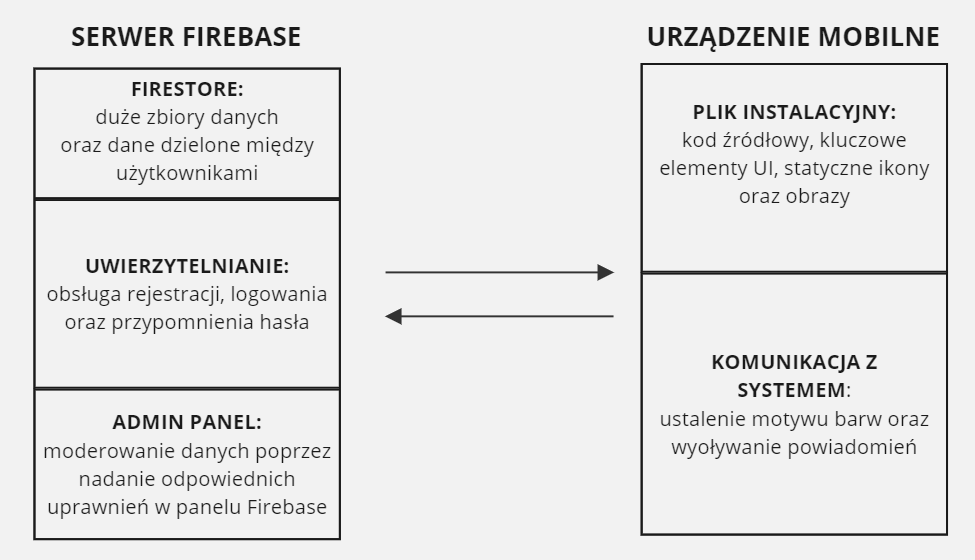
\includegraphics[width=\textwidth]{img/architektura.png}
    \caption{Architektura systemu wraz z funkcjami oraz zawartością poszczególnych elementów}
    \label{architektura}
\end{figure}
%\input{rozdzialy/przyklad_rozdzialu_3.tex}

% itd...

% ---------------------- Bibliografia -----------------------
\bibliographystyle{plain}                       % styl bibliografii
\begin{thebibliography}{3}                      % pocz +tek  +rodowiska
    \addcontentsline{toc}{chapter}{Wykaz literatury}    % dodaje bibliografi + do spisu tre +ci
    \small
    % przyk +adowy wpis
    \bibitem{Rymkiewicz}
    Olga Rymkiewicz, https://olgarymkiewicz.pl/model-4c-czyli-skad-sie-bierze-odpornosc-psychiczna/, (data dostępu 03.12.2023 r.).

    \bibitem{coaching}
    Opracowanie zbiorowe: \emph{Coaching eXtra 3/2021}, Burda Publishing Polska, 09.2021.


\end{thebibliography} % dodanie pliku bibliografii
% -----------------------------------------------------------

%------------------------------------------------------------
%	Dodanie wykazu rysunk�w oraz tabeli

\renewcommand{\baselinestretch}{1.0}\normalsize	% interlinia w sekcji wykaz�w
\addcontentsline{toc}{chapter}{\listfigurename}	% dodanie wykazu rysunk�w do spisu tre�ci
\listoffigures									% generacja wykazu rysunkw

\addcontentsline{toc}{chapter}{\listtablename}	% dodanie wykazu tabel do spisu tre�ci
\listoftables									% generacja wykazu tabel
\renewcommand{\baselinestretch}{1.3}\normalsize	% powr�t do interlinii 1.5


% ---------------------- DODATKI -----------------------
% \chapter*{Dodatek A}
% \addcontentsline{toc}{chapter}{Dodatek A}
% Zale�nie od dodatku, zaleca si� dodawa� dodatki jako
% dokumenty PDF
% \includepdf{dodatki/dodatek1.pdf}

% -----------------------------------------------------------
\end{document}
%------------------------------------------------------------
			 	%	Koniec pracy dyplomowej  %
%------------------------------------------------------------
